\subsection{Extensions (non-linear and multinomial)}

\textbf{Non-linear}\sidenote{Non-linear relationship} functions that can't be separated by a line can still be handled by using linear machinery. The basic idea for that is to transform the data in advance, leading to the following formula:
\begin{align*}
  \mathbb{M}_\mathbf{w}(\mathbf{d}) = \sum_{k=0}^b \mathbf{w}[k]\ \phi_k(\mathbf{d})
\end{align*}
\begin{itemize}
  \item Data in non-linear relationships is transformed \textit{before} applying the linear machinery.
  \item For that, apply "basis functions" $\phi_k$ like $\phi_0(x) = 1$, $\phi_1(x) = x$, $\phi_2(x) = x^2$, etc.
\end{itemize}

For the case of \textbf{multinomial regression}\sidenote{Multinomial regression}, we look at the problem where categorical data is not binary. As a solution for $n$ possible classes, we can split the decision into $n$ models (per class $i$ one model, classifying as "is class $i$" or "is not class $i$"). Those can then be combined back again into one model.

\begin{figure}[H]
  \centering
  \begin{subfigure}{0.7\textwidth}
    \centering
    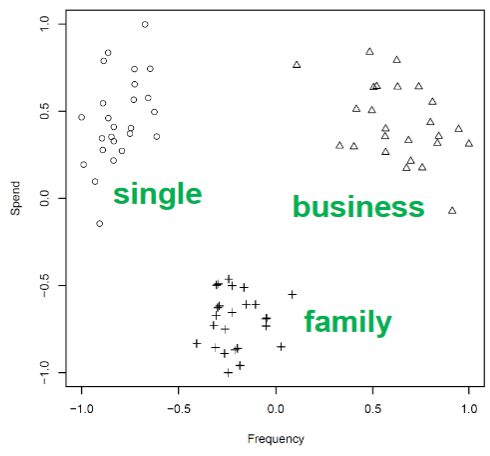
\includegraphics[width=0.4\textwidth]{assets/regression/lr__multi_problem.png}
    \subcaption{Original problem}
  \end{subfigure}
  \vspace*{0.5cm}

  \begin{subfigure}{0.7\textwidth}
    \centering
    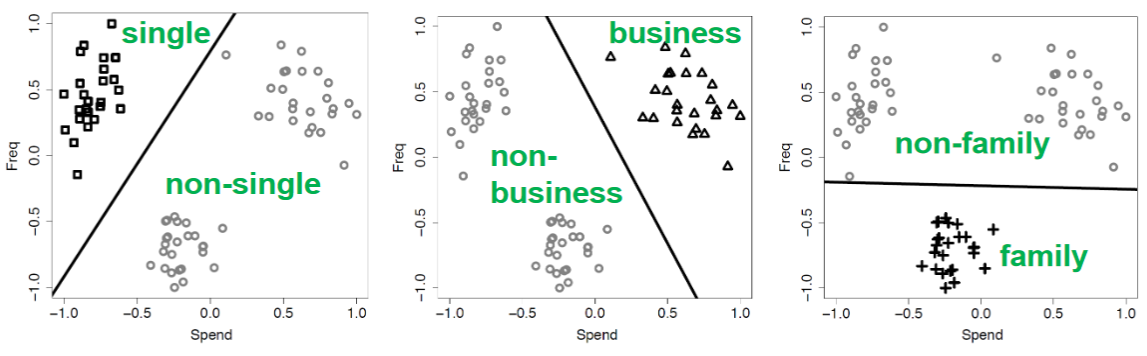
\includegraphics[width=1\textwidth]{assets/regression/lr__multi_binary.png}
    \subcaption{Binary classification}
  \end{subfigure}
  \vspace*{0.5cm}

  \begin{subfigure}{0.7\textwidth}
    \centering
    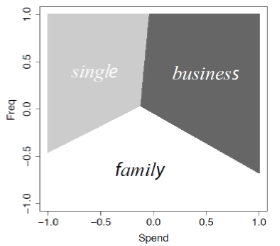
\includegraphics[width=0.4\textwidth]{assets/regression/lr__multi_sol.png}
    \subcaption{Resulting model (multinomial classification)}
  \end{subfigure}
  \caption{Combining binary (one-versus-rest) models to multinomial regression}
  \label{fig:4_multinomial}
\end{figure}